\chapter{Observations using the PyCBC modeled search pipeline}


In this chapter, we will discuss the PyCBC modeled search pipeline designed for detecting and analyzing signals from merging binary systems of compact objects like black holes and neutron stars. It is one of the major search pipelines that is used to create catalogs of binary merger observations \cite{Usman_pycbc,Allen:2005fk}. Since the inception, this pipeline has detected $\sim$ 100 binary mergers \cite{Nitz:2021uxj,2ogc,1OGC}. The PyCBC pipeline is highly modular, allowing the user to adapt its components for different types of analyses. This includes the ability to search for different types of gravitational wave sources, handle various noise artifacts in the detector data, and perform statistical analyses to assess the significance of potential detections.

We will also discuss the key observational results from the GW catalogs produced using this pipeline as an independent analysis to the LVK results: these were the third (3-OGC) \cite{Nitz:2021uxj} and the fourth (4-OGC) \cite{Nitz:2021zwj} open gravitational wave catalogs. Finally, we will briefly discuss the astrophysical implications from the current GW observations. 

%PyCBC is an open-source software package, which allows for collaborative development and improvement by the scientific community. This openness not only fosters transparency in the data analysis methods used in gravitational wave astronomy but also encourages the adoption and adaptation of these techniques in other fields of physics and astronomy.

\section{Description of the PyCBC search pipeline}\label{sec:pycbc-pipeline}

\begin{figure}
    \centering
    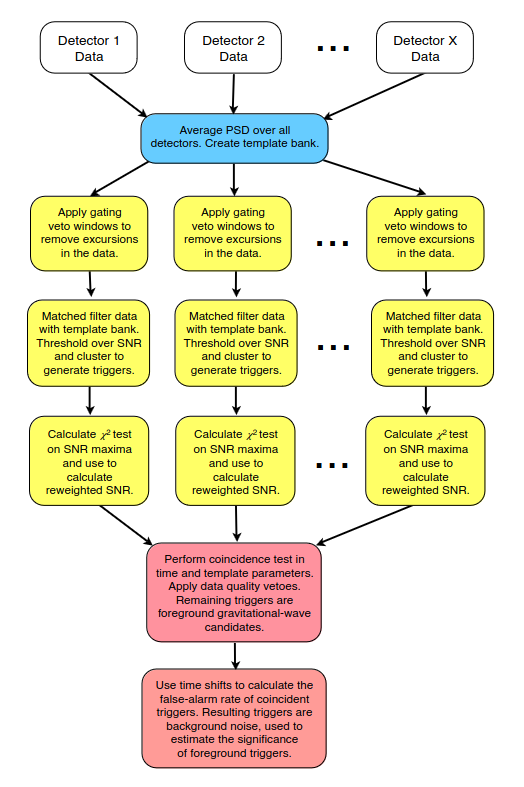
\includegraphics[width=0.75\linewidth]{figures/basic_data_analysis/search_workflow.png}
    \caption{Workflow of the PyCBC search pipeline from 2015. Constant upgrades are been made to this pipeline. In the recent version, PSD is estimated for each detector and only the one with the widest effective bandwidth is used to create a common template bank (as opposed to averaging between the detectors, as shown in the image). Loud noise transients are removed from the data from each detector using gating. Matched filtering is performed to get SNR time-series, triggers above a fixed SNR threshold are identified and clustered. Triggers are then re-weighted using the chi-squared test to suppress large tails of non-Gaussian noise. Next, candidate events are identified which pass the signal consistency checks between multiple detectors -- checks for consistency in time and template parameters. Finally, the background of noise candidates is created using time-shifts to estimate the significance of a true signal. Image credits: \cite{Usman_pycbc}}
    \label{fig:pycbc_search_workflow}
\end{figure}

\subsubsection{Inputs to the search pipeline}
There are two major inputs to the search pipeline -- 1) GW strain data from one or more detectors and 2) bank of templates corresponding to binary systems that we are searching for. We begin with strain data from the GW observatories typically sampled at a uniform sampling rate of 4096 Hz. Data segments may contain glitches or noise artefacts, which are flagged based on the information provided specific auxiliary channels \cite{LIGO:2021ppb} -- quality of a data segment is characterized by a data quality flag. Some of the relevant flags are described below \cite{LIGOScientific:2016gtq}:
\begin{enumerate}
    \item DATA: Indicates unavailability of LIGO or Virgo data.
    \item CAT1: Signifies a critical issue with a detector component, leading to major known problems. CAT1 failures are consistent across data analysis groups and such data is not openly accessible.
    \item CAT2: Represents known physical interferences, like high seismic activity, affecting the gravitational wave channel.
    \item CAT3: Indicates unexplained statistical interferences in the gravitational wave channel.
\end{enumerate}

Data-quality investigations may fail to remove some noise transients \cite{Davis:2018yrz}. Usually short duration loud transients of order of 1s having SNR $\sim (100--1000)$ can creep in the data. These transients can severely affect the sensitivity of the search by creating large number of spurious triggers. A procedure called \textit{gating} is used to mask the corrupted data around the glitch and to reduce the noise background by removing the spurious noise triggers \cite{Usman_pycbc}. 

The second input to the search is the template bank. As described in subsection (\ref{sec:MF-maximization}) the template bank consists of discrete sets of points over the intrinsic parameter space. Typically, searches are performed for quasi-circular binaries with component spins aligned to the orbital angular momentum sources emitting GW only the dominant (2,2) mode. Under these assumptions a template bank requires only four parameters -- detector frame component masses (related to the source frame masses and the cosmological redshift of the source) $m_{1,2}^{det} = (1+z)m_{1,2}$, and component spins $\chi_{1z}, \chi_{2z}$. In case of searches for eccentric or precessing sources, additional parameters need to be incorporated. 

Creating a template bank involves estimating the noise power spectral density (PSD) for each detector using Welch's method. This is done by dividing a representative period of observation into multiple 16-second blocks and estimating PSDs for each block. The median of these 16-second PSDs provides an average PSD for the detector. The detector with the widest effective bandwidth, determined by comparing PSDs across detectors, is then used to generate the template bank, as discussed below.\\  

\noindent\underline{\textit{Creating the template bank}}\\
Beginning with a blank template bank, first a random point is selected, and then a random corresponding signal within the target parameter space. We then compute the \textit{match} $m(h_i, h_{prop})$ between a given template $h_i$ and the new proposed point, given by
\begin{align}
    m(h_i, h_{\text{prop}}) &= \max_{\gamma} \Big[ \dfrac{(h_i|h_{\text{prop}}(\gamma))}{\sqrt{(h_i|h_i)(h_{\text{prop}}|h_{\text{prop}})}} \Big], \notag \\
            &= \max_{\gamma} \Big[ (\hat{h}_i|\hat{h}_{\text{prop}}(\gamma))\Big]
    \label{Eq:match-definition}
\end{align}
which maximizes the SNR over extrinsic parameters $\gamma = (d_L, \iota, \psi, \Phi_c, \alpha, \delta, t_c)$ that are not a part of the template bank. This match lies between  $0 \geq m(g,h) \leq 1$, representing the fraction of the signal's optimal SNR $(s|s) = 1$ recovered using the template $h$. We also define a quantity called the \textit{fitting factor}, as the maximum match of a signal across the complete bank 
\begin{align}
    \text{FF}(h_{\text{prop}}) = \max_i [m(h_i,h_{\text{prop}})].
    \label{Eq:fitting-factor}
\end{align}
Setting a fixed FF threshold, such as 0.97, any new point yielding a FF below this threshold suggests inadequate coverage in that region. Consequently, such a point is then incorporated into the template bank. This procedure is iteratively executed until the template bank reaches a predetermined size or the coverage limit.

The mismatch level dictates the template bank's density and requires careful calibration. A higher mismatch value results in fewer templates, potentially reducing signal SNR, while a lower value increases the number of templates, raising computational demands for matched filtering. The challenge lies in optimizing the number of templates while preserving a set minimum mismatch (1 - FF). There are numerous methods to generate a template bank which are generally categorized into three categories -- geometric lattice based methods \cite{Owen:1998dk, Babak:2006ty}, stochastic placing algorithms \cite{Harry:2009ea, Babak:2008rb}, and hybrid methods \cite{Roy:2017oul, Capano:2016dsf}. 
  

%[][][] Sampling the parameter space by computing mismatches between different waveforms require estimation of noise PSD from the data. A single PSD is used that is valid for the entire search duration to create a single template bank for a detector network. The procedure begins by separately estimating PSDs for each detector in the network using the Welch's method. Data segments of 512s is subdivided into several 16s blocks to estimate PSDs in each block -- for each segment 63 PSDs are estimated. Then the median of the several 16s PSDs is computed to average the power spectrum for the corresponding data segment. Noise PSDs from each segments are combined together as a harmonic mean for the given detector. Repeating the previous steps for each detector and finally taking the average PSD over all detector gives the PSD that is used in generating the template bank. 


\subsubsection{Matched Filtering}
At its core, the PyCBC search pipeline employs the matched-filtering technique. The inputs to the pipeline are discrete quantities -- data $s[t_i]$, templates $h[\zeta;t_i]$ described by parameters $\zeta$, and noise PSD $S_n[f_i]$. The data and the templates are transformed to their Fourier-domain equivalents $\tilde{s}[f_i]$ and $\tilde{h}[\zeta;f_i]$ respectively, using the Fast Fourier Transform (FFT) algorithm in blocks of $T_B = 512$s. The average PSD is estimated for each block using the median method as discussed previously. Computation of FFTWs is implemented via Intel's Math Kernel Libray on computer processing units (CPUs) or via Nvidia's CUDA library on graphical processing units (GPUs), these libraries are efficient in performing FFTWs in several batches in parallel.  


The discrete form of the Fourier-domain matched filtering equation is given by

\begin{align}
    \rho^2_{\zeta}[t_j] \equiv \innerprod{s}{h[\zeta]}[t_j] = 4 \Delta f \sum_{k=1}^{(N-1)/2} \dfrac{\tilde{s}[k]\tilde{h}^*[\zeta];k}{S_n[k]}e^{2i\pi j k/N},
\end{align}

giving us the matched-filter SNR time series $\rho^2[t_j]$ for a template with the parameters $\zeta$. When the SNR is above a fixed threshold (usually $\sim 5$) then a \textit{trigger} is associated to the corresponding timestamp and the triggering template. In each blocks, triggers are clustered in windows of 1s and only the loudest trigger is stored for further follow-up. 
%Plot distribution of ``SNR"

\subsubsection{Signal Consistency Tests}
The signal-to-noise ratio is effective for detecting stationary Gaussian noise, but less so with real detector noise that includes transient artifacts -- loud, short duration glitches can produce high SNRs. The PyCBC pipelines performs multiple signal consistency test to differentiate triggers due to noise artefacts and astrophysical signals, which are discussed below.\\

\noindent\underline{\textit{1. Mitigating noise artefacts}}\\

Data quality checks and gating vetoes remove only the very loud non-Gaussian noise artefacts. Many glitches are still present in the data that contribute to long tails of the SNR distribution which reduces the significance of a real astrophysical event. The chi-squared test is used to distinguish noise triggers from signal triggers which typically requires intensive computation \cite{Allen:2004gu}. It demands an extra $p-$ FFT operations for each SNR time series FFT calculation, corresponding to each frequency bin. The PyCBC pipeline, however, only computes the reduced chi-squared $\chi^2_r = \chi^2/(2p-2)$ with $p$ frequency bins at clustered trigger times in the SNR series, using an optimized frequency integral rather than FFTs. This method is more efficient unless there's poor data quality with many triggers, where FFT is faster. The matched filter SNR is then re-weighted according 
\begin{align}
    \hat{\rho}_{\zeta} = \left\{
    \begin{aligned}
        &\dfrac{\rho_{\zeta}}{[(1+(\chi_r^2)^3)/2]^{1/6}},  &\text{if}\hspace{0.2em}  \chi_{r}^2 > 1, \\
        & \rho_{\zeta}, & \text{if} \hspace{0.2em} \chi_{\zeta}^2 \leq 1,
    \end{aligned}
    \right.
\end{align}
where $\hat{\rho_{\zeta}}$ is called the \textit{re-weighted SNR} or the \textit{new-SNR}.\\

\noindent\underline{\textit{2. Coincidence between multiple detectors}}\\

To minimize the number of false alarms, the PyCBC pipeline ensures that a potential event is detected with consistent parameters across at least two detectors \cite{Davies:2020tsx}. This involves a \textit{coincidence} test on triggers after vetoing glitches. For a two-detector network, signals must be detected in both detectors within a 15 ms window, allowing for travel time and timing errors. The pipeline stores the difference in arrival times $\delta t = t_a - t_b$ and phase of the gravitational waveform $\delta \Phi = \Phi_a - \Phi_b$ for different detector pairs labelled by $a, b$. Under the assumption noise is uncorrelated between any two detectors, the distribution of noise triggers over ($\delta t, \delta \Phi$) will be random and is expected to be uniform. The same distribution for a population of astrophysical signals will have predictable but a non-trivial distribution which is pre-computed using simulated injections and stored as a lookup table for the next stages \cite{Nitz:2017svb}. The distribution of signal amplitude $\mathcal{A}_{ab} = A_{a}/A_b$ ratios across two detectors would vary for noise versus signal coincidences, as these ratios are influenced by the source's sky position and polarization angle. 

For the intrinsic parameters, the PyCBC pipeline requires exact-match coincidence, meaning triggers from each detector must have identical template parameters $\zeta$ (masses and spins). The exact-match condition is especially useful for complex gravitational waveforms, like those from spinning neutron stars or black holes, or high-mass waveforms. and has shown a noticeable improvement in search sensitivity \cite{Nitz:2017svb}. 

A coincident trigger for a given detector $a$ is described by the set $\vec{\kappa}$ of parameters including: the trigger SNR $\rho^a_{\zeta}$, reduced chi-squared value $\chi^2_{r,a}$, the triggering template's parameters $\zeta$, and the distance  $\sigma_a$ at which the SNR equals to a reference value, and multiple detector quantities like amplitude ratio $\mathcal{A}_{ab}$, time difference $\delta t_{ab}$ and phase difference $\delta\Phi_{ab}$ for $a \neq b$
\begin{align}
    \vec{\kappa} = \left\{ \rho^a_{\zeta}, \chi^2_{r,a}, \sigma_a, \zeta, \mathcal{A}_{ab}, \delta t_{ab}, \delta \Phi_{ab} \right\}.
\end{align}

Coincident triggers passing the consistency tests are ranked using a ranking statistic which we discuss in brief next.

\subsubsection{Ranking the candidates}
The optimal detection statistic is expressed as the ratio of event rate densities for signal $r_s(\vec{\kappa})$ and noise $r_n(\vec{\kappa})$ triggers described by  parameters $\vec{\kappa}$
\begin{align}
    \Lambda(\vec{\kappa}) = \dfrac{r_s(\vec{\kappa})}{r_n(\vec{\kappa})},
\end{align}
suggesting the problem is equivalent to finding the trigger rate densities. We define the coincident \textit{ranking statistic} $\mathcal{R}$ as the log of the optimal detection statistic
\begin{align}
    \mathcal{R}(\vec{\kappa}) = \log r_s(\vec{\kappa}) - \log r_n(\vec{\kappa}).
\end{align}
with the trigger densities given by 
\begin{align}
    r_s(\vec{\kappa}) &= \mu_s \dfrac{\sigma_{\min}^3}{\sigma_{\text{ref}}}p(\Omega|S),\\
    r_n(\vec{\kappa}) &= p(\Omega|N)A_{{a}}\prod_a r_{n,a}(\hat{\rho},\zeta),
\end{align}
for signal and noise respectively. We now briefly explain all the terms in involved in the trigger densities and refer the reader to \cite{Davies:2020tsx} for their detailed derivations: \\
$\bullet$ Signal trigger density: For each coincident trigger, the rate of triggers is proportional to the sensitive volume $\sigma_{\min}^3$ of the least sensitive detector. This sensitive volume is normalized by a reference volume $\sigma_{\text{ref}}^3$, which represents the average sensitivity of the network. The rate of signals is also proportional to the number of astrophysical events per volume per time, $\mu_s$. Final piece is to include the likelihood of having a signal coincidences $p(\Omega|S)$ with between the parameters $\Omega = (\mathcal{A}_{ab},\delta \Phi_{ab}, \delta_{ab})$.\\
$\bullet$ Noise trigger density: Assuming the noise in each detector {$a$} involved, is independent, the single-detector noise trigger rates for a given template $r_{n,a}(\hat{\rho})$ are multiplied together to get the rate of noise coincidences within the time window $A_a$ allowed for coincidences between multiple detectors. Similar to signal trigger density, the likelihood of noise coincidences $p(\Omega|N)$ of having the parameters $\Omega$ is established, which is assumed to be uniform across the detector network.

Finally, the coincident ranking statistic is written as
\begin{align}
    \mathcal{R}(\vec{\kappa}) = -\log A_a - &\sum_{a}\log r_{n,a}(\hat{\rho},\zeta) \\ &w- \log p(\Omega|N) + \log p(\Omega|S) + 3(\log \sigma_{\min} - \log\sigma_{\text{ref}}).
\end{align}

\subsubsection{Assigning statistical significance to candidates}
The final phase in GW event identification involves assessing the statistical significance of potential coincidences. PyCBC-based searches approach this task empirically, initially creating background triggers through \textit{time-shifts}. This involves offsetting the data from one detector relative to others by a time exceeding the light travel time between them, then detecting artificial coincidences. These coincidences constitute the search background. Then the false alarm rate (FAR) for a potential event is determined by comparing its statistical ranking with that of these simulated background triggers. This method inherently ensures that background candidates are not purely due to astrophysical signals. Repeating this process allows for the generation of noise backgrounds equivalent to over 10,000 years using just a few days of data. To reduce background noise from actual signal triggers, the PyCBC toolkit excludes triggers within a specific timeframe around high-inverse false alarm rate (IFAR) events.

\begin{figure}
    \centering
    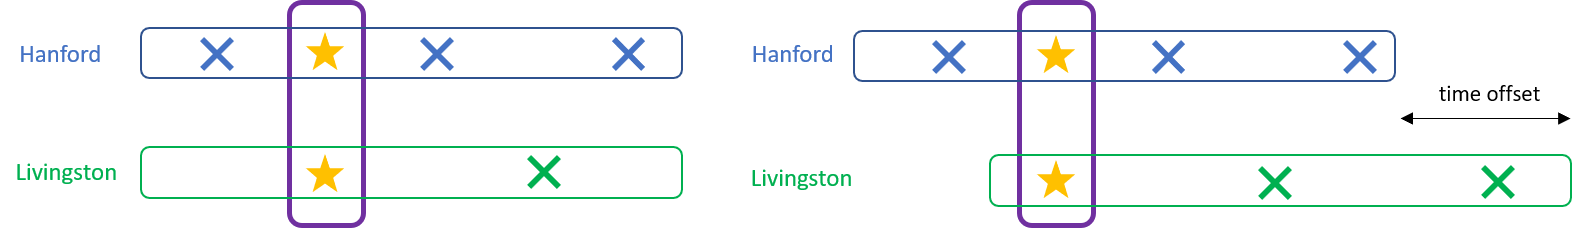
\includegraphics[width=\linewidth]{figures/current_catalogs/Time-shifts.png}
    \caption{An illustration of obtaining coincident triggers between two detectors within light travel time window (vertical) as foreground triggers (left) and background triggers (right). Background triggers are obtained by checking for coincidences for a time-shifted data (greater than light travel time) of one detector w.r.t another. This process from a few days of data can create more than 10,000 years of coincident triggers only due to noise.}
    \label{fig:Time-shifts}
\end{figure}

Nonetheless, accidental overlaps between signal and noise triggers can still occur, particularly if one is notably strong. Consequently, the PyCBC toolkit strategically removes loud triggers to lessen the impact of such astrophysical interference while maintaining an unbiased IFAR estimation. The clustering over event types dictates the calculation of false alarm rates during periods when multiple detector combinations are active. This is achieved by summing the estimated false alarm rates from all available detector combinations at the ranking statistic threshold of a candidate event \cite{Davies:2020tsx}

\begin{align}
    \text{FAR}_{\min} = \dfrac{1}{t_{\text{bg,HLV}}} + \dfrac{1}{t_{\text{bg,HL}}} + \dfrac{1}{t_{\text{bg,HV}}} + \dfrac{1}{t_{\text{bg,LV}}},
\end{align}
where $t_{\text{bg}}$ is the time-shifted total time analyzed by a given detector combination.

As an example, suppose LIGO Livingston and Virgo detect an event with a ranking statistic of 10, leading to an estimated false alarm rate (FAR) of about 1 per year (in O2 run). If LIGO Hanford's data isn't accessible at that moment, the FAR remains as is. However, if LIGO Hanford is operational and is not been part of a more significant coincidence, then the FAR for this LV event is combined with the FARs of HL (50 per year), HLV (0.8 per year), and HV (2 per year) coincidences, all at the same ranking statistic. This results in a cumulative FAR of approximately 54 per year. Essentially, this method diminishes the importance of detections by less sensitive detector pairings when more sensitive options are functioning.

\subsubsection{Sensitivity of a search}
Given a population of astrophysical signals, the population-averaged \textit{sensitive time-volume} for a search is defined as,
\begin{align}
    \langle VT \rangle = \int dz d\theta \dfrac{dV_c}{dz}\dfrac{1}{1+z}p_{\text{pop}}(\theta) f(z,\theta)T_{\text{obs}},
    \label{Eq:Sensitive-VT-generic}
\end{align}
where $dV_c/dz$ is the differential co-moving volume, $p_{\text{pop}}$ is the distribution of binary parameters $\theta$ predicted by the given astrophysical population, $f(z, \theta)$ is the detection probability for a signal with $\theta$ parameters at redshift $z$, and the observation duration of the search $T_{\text{obs}}$. Assuming that the Universe follows a Euclidean geometry, implies the redshift distribution $p(z)$ follows the star formation rate convolved with an inverse time delay model, and is written as 
\begin{align}
    p(z) = \dfrac{dV_c}{dz} \dfrac{\Psi(z)}{(1+z)V_0},
\end{align}
where $\Psi(z)$ is the specific star formation rate from \cite{Madau:2016jbv} (as shown in the Fig. \ref{fig:SFR}), and $V_0$ is the volume corresponding to the maximum redshift $z_{\max}$ of injections, given by
\begin{align}
    V_0 = \int_0^{z_{\max}} \dfrac{dV_c}{dz} \dfrac{\Psi(z)}{1+z} dz.
\end{align}
\begin{figure}
    \centering
    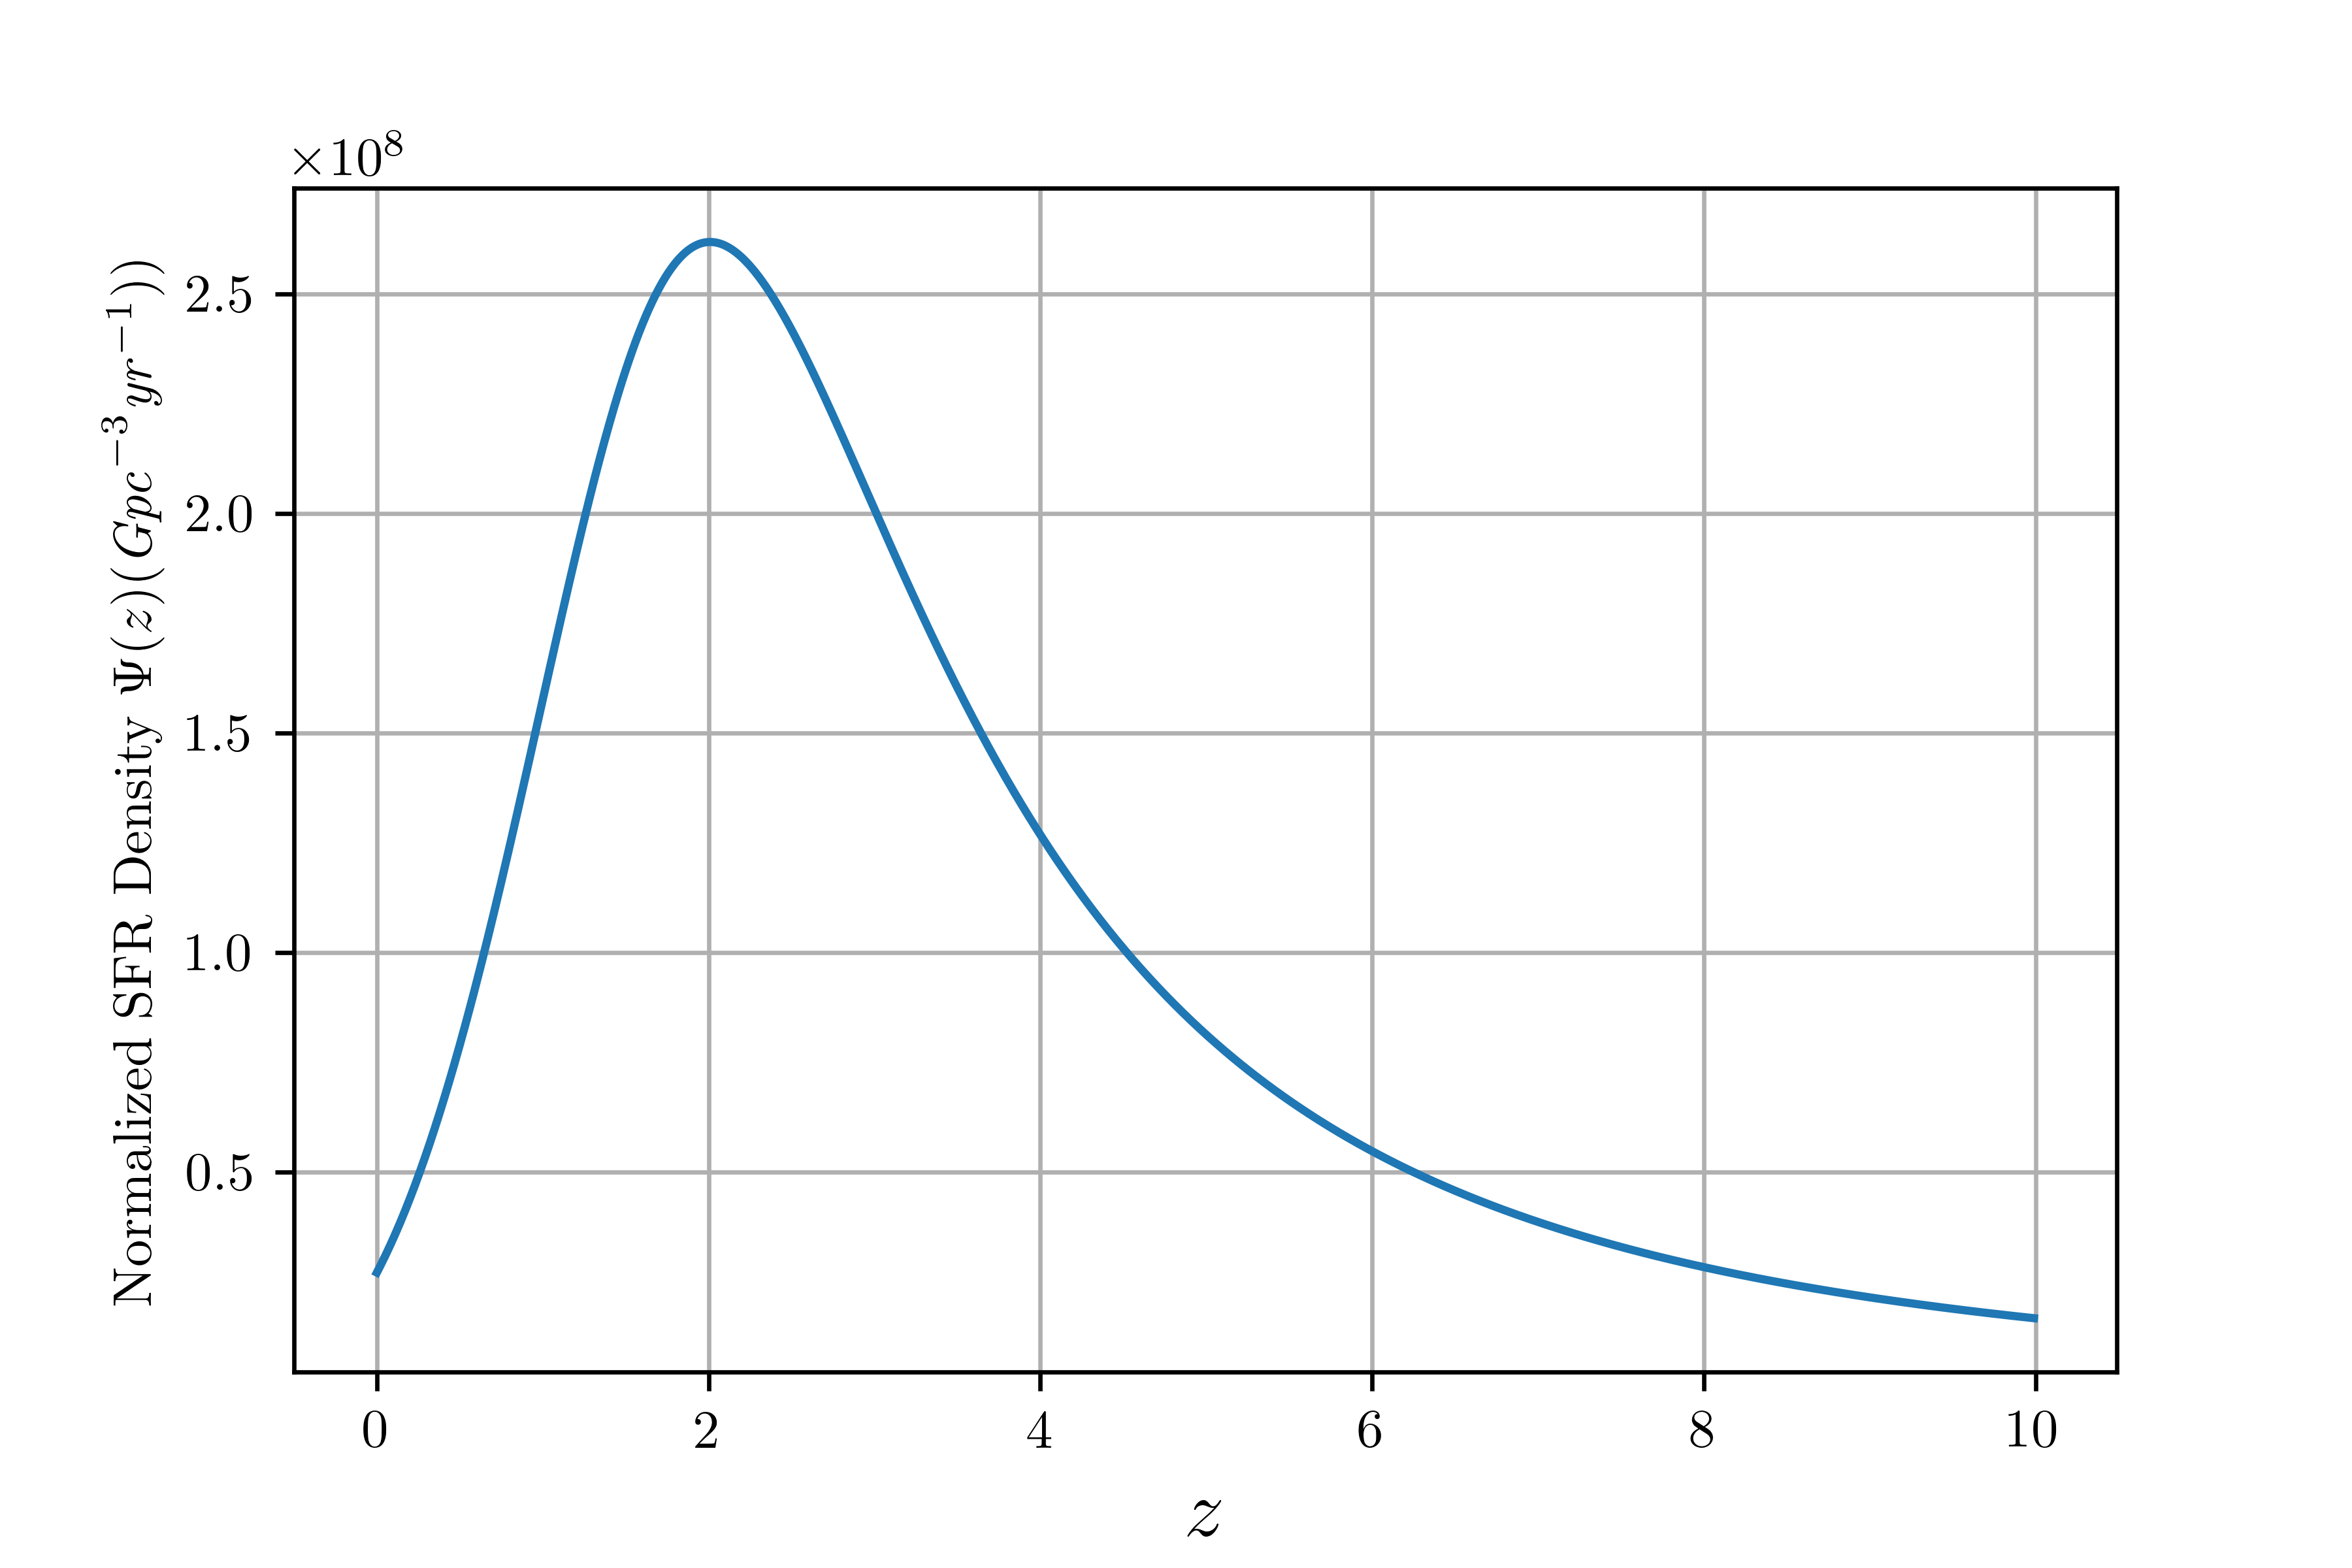
\includegraphics[width=0.8\linewidth]{figures/basic_data_analysis/SFR.png}
    \caption{Normalized star formation rate convolved with the inverse time delay model as a function of redshift \cite{Madau:2016jbv}}
    \label{fig:SFR}
\end{figure}

The sensitive time-volume $\langle VT \rangle$ in Eq. (\ref{Eq:Sensitive-VT-generic}) is evaluated via Monte Carlo integration using a large number of simulated signals \cite{Tiwari:2017ndi}, $N_I$, distributed according to the astrophysical distribution $p_{\text{pop}}$ and recovering injections from detector data below a specified false alarm rate $\mathcal{F}$
\begin{align}
    \langle VT\rangle  \approx \dfrac{V_0T_{obs}}{N_I} \sum_{i=1}^{N_I} \Theta(\mathcal{F}|\mathcal{F}_i),
    \label{Eq:generic-MC-integral}
\end{align}
where the $i^{th}$ injection having false alarm rate $\mathcal{F}_i$ will be recovered or missed completely according to the step function $\Theta(\mathcal{F}|\mathcal{F}_i) = 1$ if $\mathcal{F}_i \leq \mathcal{F}$ and zero otherwise. Typical threshold for FAR is chosen to be less than ($10^{-3}-10^{-2}$)/Yr. 

However, this kind of analysis have two shortcomings: 1) Multiple injection runs are required to assess the sensitive volume for various population models. 2) Since the distribution of injection increases with redshift and is independent of $\theta$, most of the injections do not contribute to the sensitive volume as they are placed at redshifts where their detection is unfeasible. 

To overcome these two challenges, injections are performed using detector based parameters $\theta^{det}$ using distributions $p_{\text{inj}}$ that will allow the search pipeline to retrieve adequate number of injections where $p_{\text{pop}}$ is significant. Also, the placement of these injections in terms of the redshift is made sure such that they occur in locations where the recovery probability, denoted as $f(z, \theta)$, is not zero. The sensitive volume using generic injection sets can be computed in the similar way as Eq. (\ref{Eq:generic-MC-integral}) but using a weight $w$ for each injection
\begin{align}
    w_i = \dfrac{p_{\text{pop}}(\theta_i)}{p_{\text{inj}}(\theta_{i}^{det})}\dfrac{1}{J_i},
    \label{Eq:MC_weights}
\end{align}
where $J_i$ is the Jacobian which maps the distribution from the detector frame parameters $\theta^{det}_i$ to the source frame $\theta_i$ via
\begin{align}
    J_i = \Bigg(\dfrac{\partial\theta_i}{\partial\theta_{i}^{det}} \Bigg)_i.
\end{align}
Finally, the sensitive $\langle VT \rangle$ is estimated using Eqs (\ref{Eq:generic-MC-integral}) and (\ref{Eq:MC_weights}), assuming $N_{I,\mathcal{F}}$ number of recovered injections below the FAR threshold $\mathcal{F}$ from the distribution $p_{\text{inj}}(\theta^{det})$
\begin{align}
    \langle VT \rangle = V_0T_{obs}\dfrac{N_{I,\mathcal{F}}}{N_I} \dfrac{\sum\limits_{i \in \text{rec}}w_i}{\sum\limits_{i\in \text{total}}w_i},
\end{align}
and the error on this estimate is 
\begin{align}
    \dfrac{\delta \langle VT \rangle}{\langle VT \rangle} = \dfrac{\sqrt{\sum\limits_{i\in \text{rec}}w_i^2}}{\sum\limits_{i \in \text{rec}}w_i}.
\end{align}

To quantify search sensitivity for a given system (i.e fixed source parameters), we define the \textit{sensitive distance} -- the radius of a sphere with volume $\langle V \rangle$, corresponding to the average distance at which a given system can be recovered by the search. Since the amplitude of GWs scales as the chirp mass of the system, if we assume a binary with $\mathcal{M}_0$ is detectable up to a distance of $r_0$, then another binary with a chirp mass $\mathcal{M}$ can be detected at a distance that can be approximated by the following relationship:
\begin{align}
    r_i = r_0 (\mathcal{M}_i/\mathcal{M}_0)^{5/6}.
\end{align}
The above approximation is valid only to the first order, and assumes the sources are distributed
uniform in co-moving volume. 

\section{Current observations of gravitational-wave events}

From the initial detection in 2015 up to the completion of the third observation run by the Advanced LIGO and Virgo detectors in 2020, approximately 100 compact binary events have been recorded \cite{Nitz:2021zwj,LIGOScientific:2021djp,Olsen:2022pin}. The precise count of these events varies depending on the specific search pipeline utilized for identifying GW events. Beyond PyCBC, there are three other pipelines used for archival GW searches: GstLAL \cite{Messick:2016aqy, Cannon:2020qnf}, Multi-Band Template Analysis (MBTA) \cite{Adams:2015ulm,Aubin:2020goo} and IAS pipeline \cite{Olsen:2022pin,Mehta:2022pcn}. 

These pipelines are distinguished by their unique technical and configuration features. One notable difference lies in the approach each pipeline uses to determine the False Alarm Rates (FARs) for candidates. GstLAL, for instance, assesses candidates against a global background encompassing the entire observation duration. In contrast, pipelines like MBTA, and PyCBC rely on a local background derived from a shorter typical period, ranging from one to several weeks. These various pipelines have contributed to the publication of different GW catalogs \cite{Nitz:2021zwj,LIGOScientific:2021djp,Olsen:2022pin}. In this section, we aim to succinctly spotlight the key observational findings from the third and fourth open gravitational wave catalogs (OGCs) and discuss the astrophysical insights derived from these observations.

\subsection{The 4-OGC and 3-OGC catalogs}
The open gravitational wave catalogs represent a series of independent studies \cite{Nitz:2021uxj, Nitz:2021zwj}, analyzing publicly accessible data from the LIGO and Virgo observatories \cite{Vallisneri:2014vxa,Abbott:2019ebz}. This analysis involves searching for a wide range of binaries and following up the significant events with an extensive parameter estimation. 

\subsubsection{Observation period} 
In the latest fourth edition of the OGC, we have performed a deep archival search of all the public data from the years 2015 to 2020 \cite{Nitz:2021zwj}, incorporating all the observational runs conducted so far (O1, O2, O3a, O3b). This latest catalog builds upon the findings of the 3-OGC catalog \cite{Nitz:2021uxj}, notably expanding its scope by including data from the second part of the third observing run, O3b. During the entire O3 observation period, there were 152 days where all three detectors were operational simultaneously, and approximately 200 days when both LIGO detectors were active. The analysis encompasses all instances where multiple detectors were observing simultaneously. Additionally, events are identified in scenarios where only one of the LIGO detectors, either LIGO-Livingston or LIGO-Hanford, was operational. However, data from periods when only Virgo is online is excluded due to its reduced range and the substantial presence of non-Gaussian transient noise.

\begin{table}
  \begin{center}
    \caption{Analyzed time in days for different global network observing scenarios. The abbreviations H, L, and V are used for the LIGO-Hanford, LIGO-Livingston, and Virgo observatories, respectively. Each time period is exclusive of the others. Some data is excluded from the full public dataset due to analysis requirements ($O(1)\%$). However, data around GW170608 and GW190814 which was made available separately from the bulk data release is included \cite{Vallisneri:2014vxa}.}
    \label{table:4ogc-timeline}
\begin{tabular}{rrrrrrrr}
Observation & HLV & HL & HV & LV & H & L & V \\\hline
O1 \vline& - & 48.6 & - & - & 27.6 & 17.0 & - \\
O2 \vline&15.2 & 103.3 & 1.7 & 2.2 & 37.8 & 33.0 & 1.7 \\
O3 \vline&152.0 & 49.5 & 31.7 & 38.9 & 10.3 & 9.9 & 25.0 \\
All \vline&167.2 & 201.4 & 33.4 & 41.1 & 75.6 & 59.9 & 26.7 \\
\end{tabular}
  \end{center}
\end{table}

\begin{figure}
    \centering
    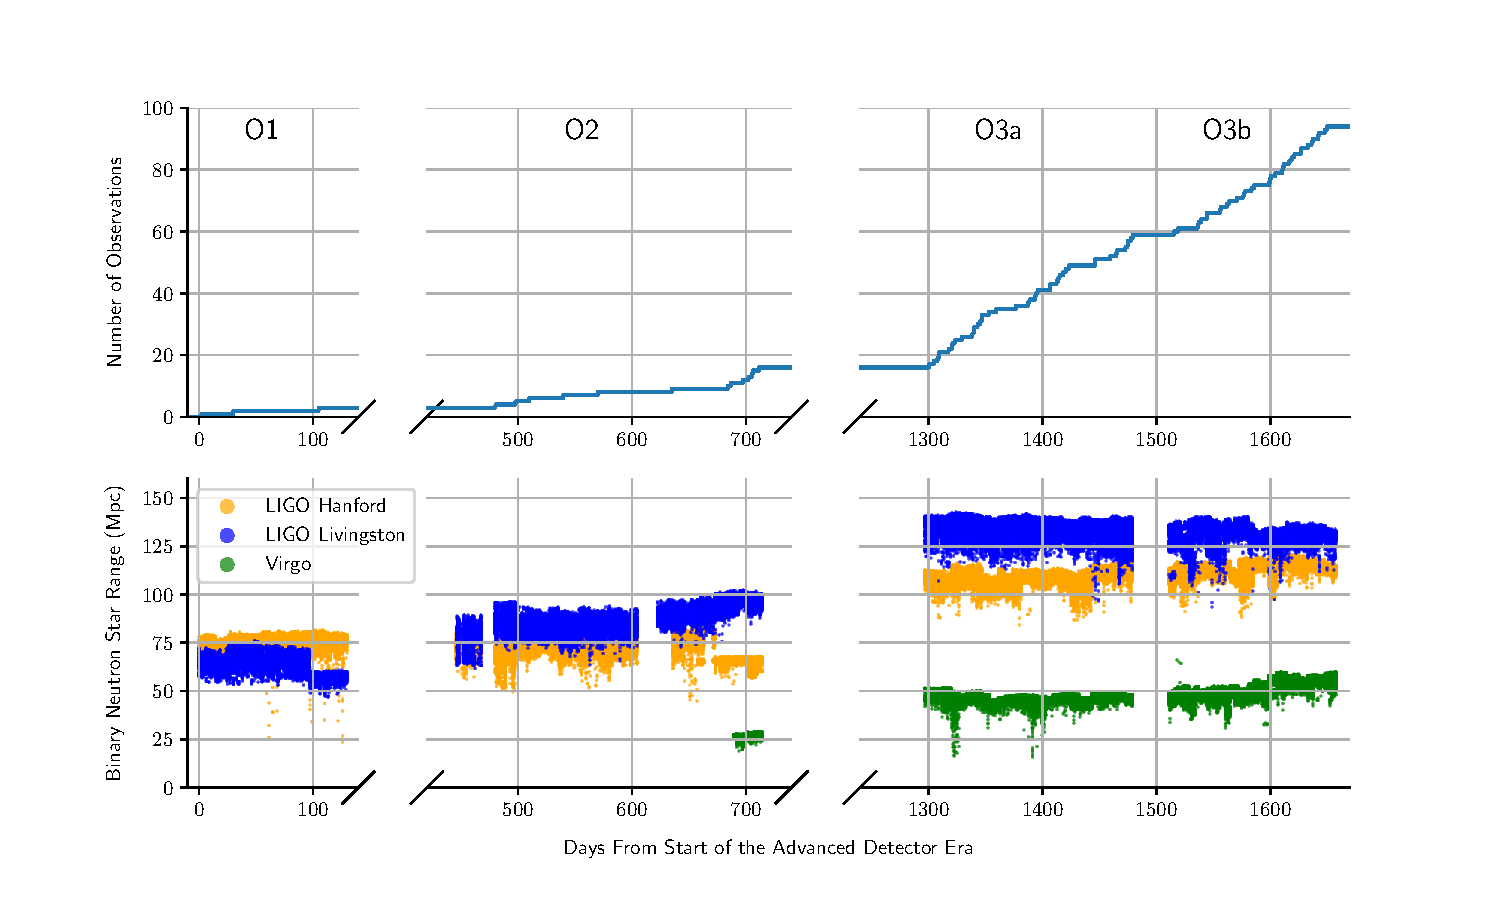
\includegraphics[width=\linewidth]{figures/current_catalogs/range.pdf}
    \caption{In the top panel shows the cumulative number of binary merger observations as a function of days since the commission of advanced GW detectors. The bottom panel shows the range of various detectors LIGO Hanford (Blue), LIGO Livingston(orange) and Virgo (green ). The range for a given detector is defined as the distance at which a fiducial 1.4-1.4$M_{\odot}$ BNS systems (averaged over orientation and sky location) would give an SNR of 8. Three different observing periods are shown -- O1(left), O2(middle) and O3a+O3b(right).}
    \label{fig:4OGC-range}
\end{figure}



\begin{figure}
    \centering
    \includegraphics[width=\linewidth]{figures/current_catalogs/4OGC.png}
    \caption{Spectrograms of all the BBH, NSBH and BNS events from the fourth open gravitational wave catalog. The catalog features observations between 2015-2020 and includes a total of 94 observations: 90BBHs, 2NSBHs and 2BNSs mergers. Image credits: Alexander H. Nitz}
    \label{fig:4OGC-spectrograms}
\end{figure}

\subsubsection{Search region}
For source identification across a wide range of parameter space, including component masses and spins a discrete template bank is used for this catalog, as depicted in Fig. \ref{fig:4OGC-bank} (same as the one utilized in the 3-OGC analysis \cite{Nitz:2021uxj}). The bank is created using stochastic placement algorithm \cite{Harry:2009ea}. For low mass-ratio, low-spin binary black holes (BBH), a specialized bank is designed to recover over 99.5\% of the signal SNR. Additionally, there are banks for binary neutron stars (BNS), neutron star-black hole (NSBH) systems, and a broad-parameter BBH bank targeting an SNR recovery of more than 97\%. The templates are specifically designed to capture signals from non-precessing, nearly circular sources. The search focuses on the primary-mode gravitational wave signal and excludes higher-order mode effects.

To model the gravitational wave signals, a mix of waveform approximations are used: \approximant{TaylorF2} for BNS sources \cite{Sathyaprakash:1991mt,Droz:1999qx,Blanchet:2004ek,Faye:2012we}, \approximant{SEOBNRv4\_ROM} for BBH and NSBH \cite{Taracchini:2012ig,Bohe:2016gbl}, and \approximant{IMRPhenomD} for targeted BBH searches \cite{Husa:2015iqa, Khan:2015jqa}.


\begin{figure}
    \centering
    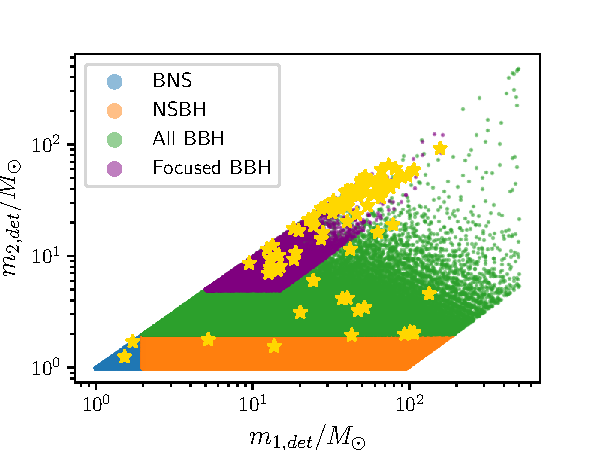
\includegraphics[width=\linewidth]{figures/current_catalogs/bank.pdf}
    \caption{ The template bank used in the 4OGC analysis described by the detector-frame component masses. The templates are categorized into different regions: binary neutron star (BNS) shown in blue, neutron star–black hole (NS-BH) in orange, binary black hole (BBH) in green, and a specialized category for BBH in purple. Each observed merger event is indicated with a star symbol on the corresponding template. We only display the template that yielded the candidate with the lowest false alarm rate for clarity in this representation.}
    \label{fig:4OGC-bank}
\end{figure}


\subsubsection{Notable binary merger events}
We will highlight a few notable confident events found to date and refer the reader to \cite{Nitz:2021zwj} for the complete list of the observed events from the 4OGC analysis.\\

\noindent\underline{\textit{Binary black holes}}
\begin{itemize}
    \item GW150914: This was the first direct detection of gravitational waves, observed on September 14, 2015. It was a merger of two black holes and confirmed a major prediction of Einstein's theory of general relativity.
    \item GW190412: The most unequal mass binary black hole was observed on 12 April, 2019. Due to this significant mass difference, GW190412 provided the first clear observation of \textit{higher-order modes} in gravitational wave signals.  
    \item GW190521: Observed on May 21, 2019, this event was remarkable for being the first detection of an 
    \textit{intermediate-mass} black hole (IMBH), resulting from the merger of two smaller black holes. It opened a new window into a previously unobserved class of black holes. The ring-down analysis of GW190521 points to the presence of a less dominant mode.
    \item GW200129: This event, detected on January 29, 2020, is particularly significant because it showed strong evidence of \textit{orbital precession}. This was the first black hole merger identified as having a large recoil velocity for the final black hole left behind after the merger.
\end{itemize}

\noindent\underline{\textit{Neutron star binaries}}
\begin{itemize}
    \item GW170817: Detected on August 17, 2017, this event was significant for being the first observation of a binary neutron star merger. It was also notable for its electromagnetic counterpart, observed across the spectrum, which marked the beginning of multi-messenger astronomy involving gravitational waves.
    \item GW190814: Detected on August 14, 2019, this event involved a collision between a black hole and a mysterious compact object of about 2.6 solar masses, which lies in the so-called ``\textit{mass gap}" between the heaviest known neutron stars and the lightest known black holes.
    \item GW200105 and GW200115: These events, detected in January 2020, were among the first confirmed detections of neutron star-black hole mergers. 
\end{itemize}






\subsection{Astrophysical implications from the current observations}
One of the primary complexities in the field of GW astrophysics is the ambiguity in interpreting observational data, which can vary based on the postulated history of the merger's formation. Therefore, distinguishing the unique origins of merger events based on their observational signatures is of paramount importance.

An illustrative example is provided by the most massive GW event on record to date (GW190521), which was interpreted as a merger between two BHs with a combined mass of 150 $M_{\odot}$, with the primary BH weighing over 65 $M_{\odot}$ at a 99\% confidence level (refer to \cite{LIGOScientific:2020aai, Fishbach:2019bbm} for a perspective that a mass over 120 $M_{\odot}$ is plausible). The formation of such a massive BH through isolated binary evolution is deemed highly improbable, as it would typically be in the range of 50 $M_{\odot}$ to 120 $M_{\odot}$ — a region expected to yield no remnant due to pair-instability supernovae (PISN) \cite{Bond:1984sn, Woosley:2016hmi}. Should GW190521 indeed include a BH mass within this predicted gap, it would strongly suggest an origin different than the isolated binary star evolution.

However, drawing broader conclusions about the evolution of massive stars from singular observations requires an understanding of how typical such instances are. As the pool of GW data grows, it allows for a more detailed understanding of the properties of local binary mergers, such as the rates at which they occur and their mass distributions. Weaker constraints exist on their spin distributions and sky localizations, which could indicate potential host galaxies.

One particularly interesting discovery is that the bulk of the BBH mergers observed — 32 out of 44 systems - feature at least one BH exceeding 30 $M_{\odot}$ in mass. The prevalence of such massive BHs among GW findings, while anticipated due to selection biases, is noteworthy since electromagnetically observed systems with BHs before the era of GW detection were estimated to be less than 20 $M_{\odot}$ \cite{Tetarenko:2016uln,Miller-Jones:2021plh}. The maximum mass achievable by a BH from stellar origin is understood to be metallicity-dependent, with wind mass loss rates during the massive star phase increasing with metal content, thus reducing the final mass of the BH \cite{Vink:2001cg,Vink:2005zf}. This has led to theories that the massive BHBH mergers detected through GWs may arise from low-metallicity star formation regions or potentially from previous merger events.

The potential for gravitational wave data to reveal discontinuities, such as mass gaps or cutoffs, within the compact object mass spectrum is of significant interest for its implications on core collapse and stellar explosion physics. Differing explosion models predict varying outcomes, such as a mass gap between approximately (3--5) $M_{\odot}$ due to the dynamics of massive stellar core collapse, with others anticipating a more uniform distribution \cite{Fryer:2011cx}. GW data can thus provide valuable constraints on these theoretical models.

The advancement in detector sensitivity is starting to allow examination of the BBH population across cosmic time. The anticipated evolution of GW detector capabilities, with projects like Cosmic Explorer and Einstein Telescope \cite{Reitze:2019iox, Maggiore:2019uih}, promises to map this dependency across the span of cosmic star formation history. Such insights could enhance our comprehension of the Universe's chemical evolution and its correlation with unresolved questions. 


%Since the current advanced LIGO and advanced VIRGO detectors went online 